\section{Auswertung}
\label{sec:Auswertung}
\subsection{Bestimmung der mittleren Reichweite}
Zweite Gerade Messung 2:  [-1235.2008984    871.99237113]  +/-  [ 45.25758979  28.04695956]
Dritte Gerade Messung 1:  [-4162.69745858  3579.8549698 ]  +/-  [ 925.3436687   742.81680245]

Aus dem in Abb.\ref{fig:Energie} mittels \eqref{eqn:gerade} gefitteten Ausgleich der ersten Messung erhält man die Parameter: $a_1 = \SI{-2.11 \pm 0.06}{\mega\eV}$, $b_1=\SI{4.06 \pm 0.03}{\mega\eV}$. Entsprechend liefert die zweite Messung $a_2 = \SI{-2.67 \pm 0.09}{\mega\eV}$, $b_2 = \SI{4.06 \pm 0.03}{\mega eV}$. Der Abstand der Sonde zum Zähler ist im ersten Durchlauf $x_1 = \SI{23}{\milli\meter}$, im zweiten $x_2 = \SI{29}{\milli\meter}$. Die Energiesteigung ergibt sich somit zu:

\begin{align*}
  -\frac{\symup{d}E_1}{\symup{d}x}=\SI{91.7 \pm 2.6}{\mega\eV\per\meter} \\
  -\frac{\symup{d}E_2}{\symup{d}x}=\SI{92.0 \pm 3.1}{\mega\eV\per\meter}.
\end{align*}

Aus der Bethe-Bloch-Formel der Reichweite ergibt sich somit
\begin{align*}
  R_1 = b_1/\frac{\symup{d}E_1}{\symup{d}x} = \SI{0.04\pm 0.01}{\meter} \\
  R_2 = b_2/\frac{\symup{d}E_2}{\symup{d}x} = \SI{0.04\pm 0.01}{\meter}.
\end{align*}

\begin{equation}
  f(x) = a\cdot x +b
  \label{eqn:gerade}
\end{equation}

\begin{figure}
  \centering
  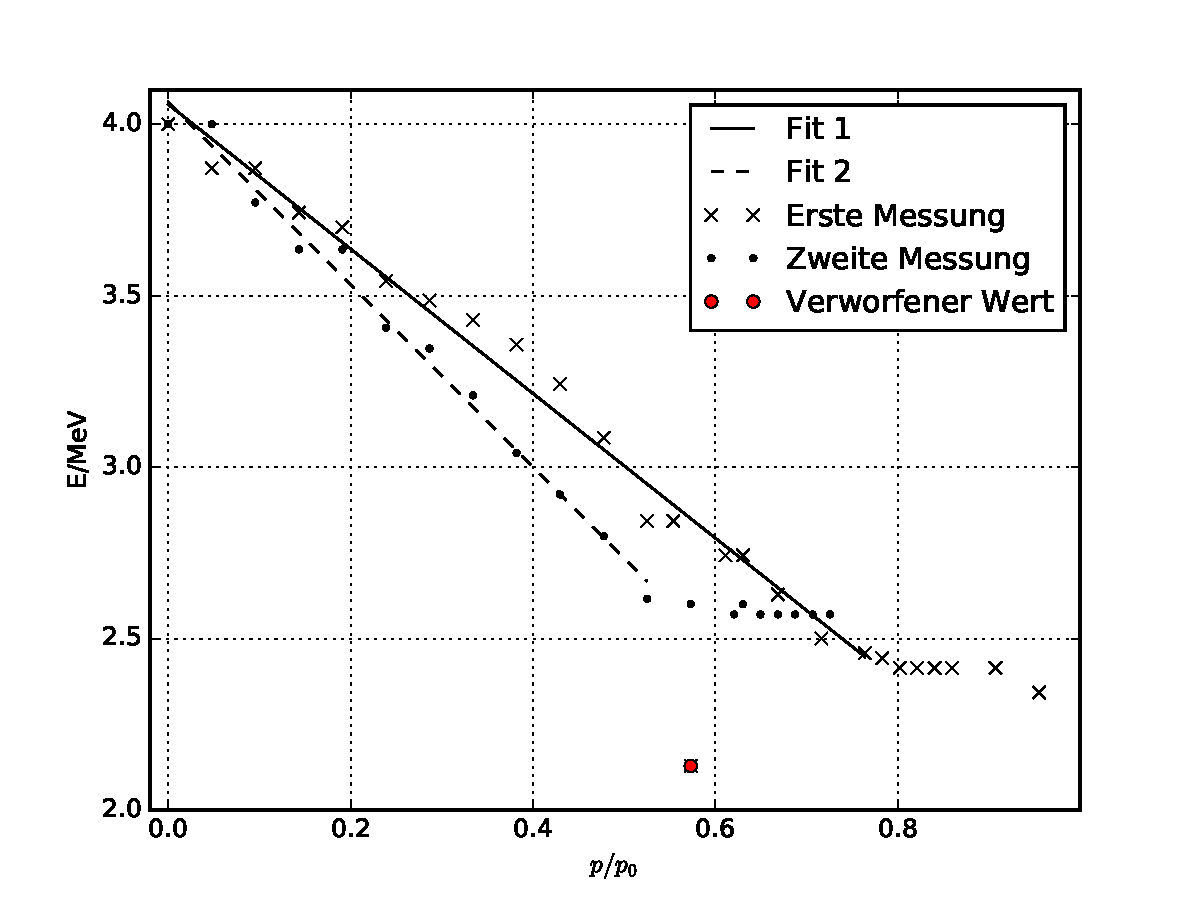
\includegraphics[height=6cm]{plots/Energie.pdf}
  \caption{Energie der gemessenen $\alpha$-Teilchen aufgetragen gegen den relativen Druck $p/p_0$}
  \label{fig:Energie}
\end{figure}

Für die Plateau-Phase erhält man eine gemittelte Zählrate von $f_1 = \SI{580\pm5}{\hertz}$, bzw. $f_2 = \SI{377\pm9}{\hertz}$. Wie Abb. \ref{fig:Rate} zu entnehmen, wurde für den Berreich des stärksten Abfalls ein linearer Fit gemäß \eqref{eqn:gerada} druchgeführt. Die Parameter hierfür sind:
\begin{align*}
  a_{f_1} = -\SI{4163 \pm 925}{\hertz} \\
  b_{f_1} = \SI{3580 \pm 743}{\hertz} \\
  a_{f_2} = -\SI{1235 \pm 45}{\hertz} \\
  b_{f_2} = \SI{872 \pm 28}{\hertz}
\end{align*}

\begin{figure}
  \centering
  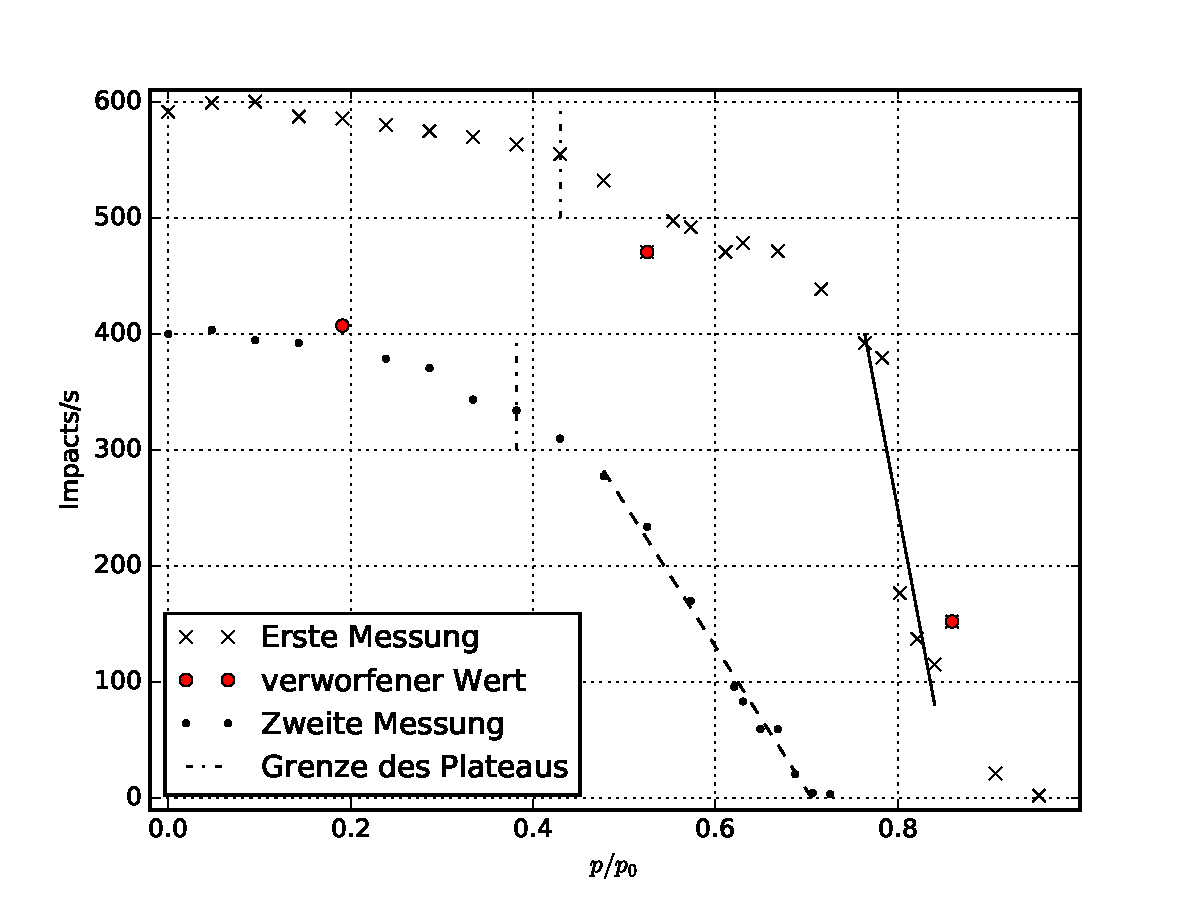
\includegraphics[height=6cm]{plots/Rate.pdf}
  \caption{Zählrate aufgetragen gegen den relativen Druck $p/p_0$}
  \label{fig:Rate}
\end{figure}

\subsection{Statistik des Zerfalls}

m:  533.9755
bins:  [ 495.8  505.2  514.6  524.   533.4  542.8  552.2  561.6  571.   580.4
  589.8]
n:  [  9.  24.  28.  40.  38.  26.  19.  13.   2.   1.]
halo i bims, 1 echter balken:  [500 509 519 528 538 547 556 566 575 585]
halo i bims, 1 gauß:  [ 19.81087747] +/- [ 1.07412195]


Die genommenen Messwerte wurden als normiertes Histogram in Abb. \ref{fig:hist} dargestellt, d.h. das Histogram wurde so normiert, dass die Summe über alle Balken 1 beträgt. Die eingezeichnete Fit-Kurve stellt eine Gauß-Normalverteilung gemäß
\begin{equation}
  G(x) = \frac{A}{\sigma\cdot\sqrt(2\pi)}e^{-0.5 {\frac{x-m}{\sigma}}^2}
  \label{eqn:gauß}
\end{equation}
dar. Hierbei ist  $\sigma=\SI{19.81 \pm 1.07}{\hertz}$ die Standardabweichung und $m= \SI{533.98}{\hertz}$ der Mittelwert der aufgenommenen Werte. Im Histogram wurden 10 Balken aufgelöst, was einer Breite von ca. $\SI{10}{\hertz}$ entspricht und somit höher auflösend gewählt wurde als die Standardabweichung.

 \begin{figure}
   \centering
   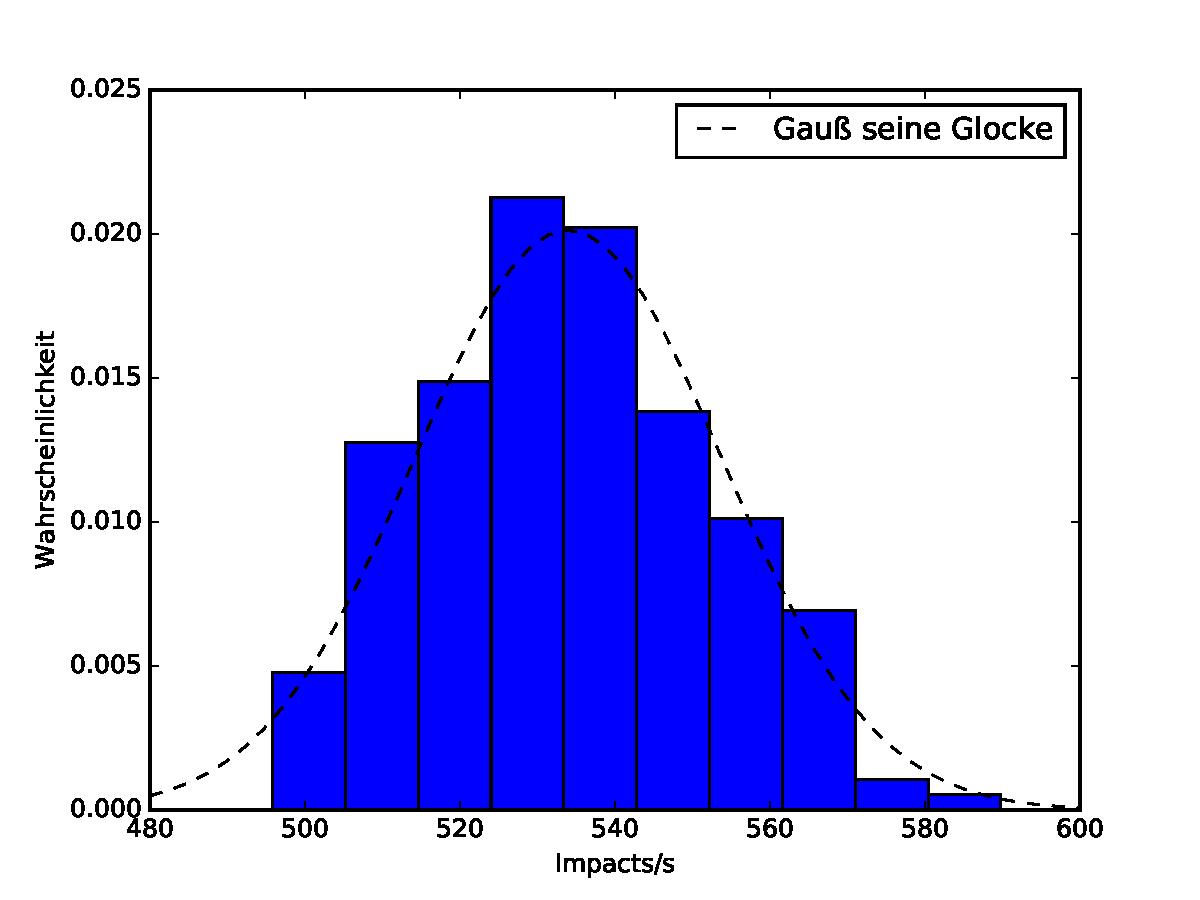
\includegraphics[height=6cm]{plots/Statistik.pdf}
   \caption{Histogram zur Zählrate}
   \label{fig:hist}
 \end{figure}
